%+TITLE: Ruptura espontánea de simetría
%+DESCRIPTION: Estudiamos vacíos que rompen simetrías globales y demostramos el teorema de Goldstone
\documentclass[11pt,a4paper]{article}

\usepackage[utf8]{inputenc}
\usepackage[T1]{fontenc}
\usepackage[spanish,es-nodecimaldot]{babel}
\usepackage{lmodern}
\usepackage{amsmath,amssymb,mathtools}
\usepackage{graphicx}
\usepackage{xcolor}
\usepackage{geometry}
\usepackage{enumitem}
\usepackage{microtype}

\geometry{margin=2.3cm}
\setlength{\parindent}{0pt}
\setlength{\parskip}{0.65em}
\setlist[itemize]{leftmargin=1.6em,itemsep=0.25em,topsep=0.25em}

\definecolor{title-red}{RGB}{165,25,20}
\definecolor{concept-green}{RGB}{20,125,45}
\newcommand{\concept}[1]{\textcolor{concept-green}{#1}}

\newcommand{\ket}[1]{\left|#1\right\rangle}
\newcommand{\bra}[1]{\left\langle#1\right|}
\newcommand{\braket}[2]{\left\langle #1\middle|#2\right\rangle}
\newcommand{\hc}{\mathrm{h.c.}}
\newcommand{\Tr}{\operatorname{Tr}}
\newcommand{\Diffs}{\mathrm{Diffs}}
\newcommand{\slashedpartial}{\not\!\partial}

\begin{document}

La interacción nuclear débil es una interacción de gauge $SU(2)$ mediada por
bosones de gauge masivos. Esto no parecería posible ya que un término de masa
para un bosón de gauge, del estilo
\[
  -\frac12m_W^2W_\mu W^\mu,
\]
no es invariante de gauge (tarea).

Por otro lado se estudiaban en materia condensada las teorías con una simetría
espontáneamente rota. La ruptura espontánea de una simetría de gauge le da masa
a los bosones de gauge, como veremos más adelante. Pero antes demostremos el
\concept{teorema de Goldstone}, según el cual la ruptura espontánea de una
simetría global implica la presencia de partículas sin masa.

¿Qué es la ruptura espontánea de la simetría? Ocurre cuando el estado fundamental elegido
no respeta una simetría de las ecuaciones de la teoría. El ejemplo estereotípico es el
ferromagnetismo.

\begin{center}
  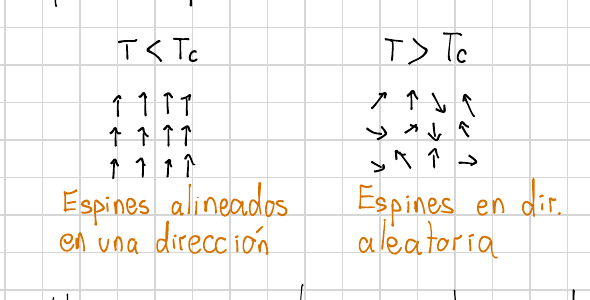
\includegraphics[width=0.56\linewidth]{figures/ferromagnetismo.png}
\end{center}

Para $T<T_c$ el sistema no es invariante bajo rotaciones. Los espines apuntan en
alguna dirección que parece privilegiada. ¡Pero sabemos que las leyes de la
física sí son invariantes bajo rotaciones! Aquí la simetría está
\concept{espontáneamente rota}.

Hagamos un ejemplo con una teoría de campo. Tomemos dos campos escalares
$\phi_1,\phi_2$ que organizamos
\[
  \phi=\frac{\phi_1+i\phi_2}{\sqrt{2}},
\]
con lagrangiano
\[
  \mathcal L
  =-\partial_\mu\phi^*\partial^\mu\phi-m^2\phi^*\phi
   -\lambda(\phi^*\phi)^2
  \equiv-\partial_\mu\phi^*\partial^\mu\phi-V(\phi).
\]

Esta teoría tiene una invariancia $U(1)$ global:
\[
  \phi\longmapsto\phi'=e^{i\alpha}\phi.
\]

Ahora supongamos que $m^2<0$ y $\lambda>0$. El campo tenderá a moverse cerca del
mínimo de potencial.

\begin{center}
  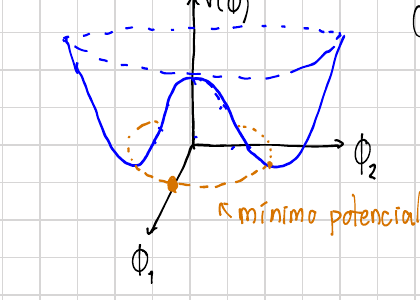
\includegraphics[width=0.40\linewidth]{figures/potencial_sombrero_mexicano.png}
\end{center}

\[
  0=\frac{\partial V}{\partial\phi}
   =m^2\phi^*+2\lambda(\phi^*\phi)\phi^*
  \qquad\Longrightarrow\qquad
  \begin{cases}
    \phi=0 & \longrightarrow \text{máximo},\\[2mm]
    |\phi|^2=-\dfrac{m^2}{2\lambda}=a^2 & \longrightarrow \text{mínimo}.
  \end{cases}
\]

El mínimo de potencial es un círculo en el plano complejo $\phi_1,\phi_2$.
Cualquier punto de ese círculo es un punto estable para el sistema. Por ejemplo
el punto $\phi_1=\sqrt2a$, $\phi_2=0$ es un mínimo, pero bajo $U(1)$
$\phi_1'=\sqrt2a\cos\alpha$, $\phi_2'=\sqrt2a\sin\alpha$. Es decir, el mínimo no es invariante y
$U(1)$ está espontáneamente rota.

Escojamos ese mínimo $\phi_1=\sqrt2a$, $\phi_2=0$ y parametricemos
\[
  \phi(x)=(a+\rho(x))e^{i\theta(x)},
\]
tal que el mínimo es $\rho=0$, $\theta=0$. El lagrangiano es
\[
  \mathcal L
  =-\partial_\mu\rho\,\partial^\mu\rho
   -(a+\rho)^2\partial_\mu\theta\,\partial^\mu\theta
   -m^2(\rho+a)^2-\lambda(\rho+a)^4.
\]

Para leer las masas hay que normalizar canónicamente los campos.
A orden cuadrático, $r=\sqrt2\rho$ y $\pi=\sqrt2a\theta$ dan
\[
  \mathcal L_2
  =-\frac12\partial_\mu r\,\partial^\mu r
   -\frac12(4\lambda a^2)r^2
   -\frac12\partial_\mu\pi\,\partial^\mu\pi.
\]
Así, $m_\pi^2=0$: este es el \concept{bosón de Goldstone}.
El modo radial tiene $m_r^2=4\lambda a^2$.
La simetría sigue presente como $\theta\mapsto\theta+\alpha$,
pero mueve el vacío elegido.

Complicemos el ejemplo, ahora con tres campos escalares y simetría $SO(3)$:
\[
  \mathcal L
  =-\frac12\partial_\mu\phi_i\partial^\mu\phi_i
   -\frac{m^2}{2}\phi_i\phi_i
   -\lambda(\phi_i\phi_i)^2,
  \qquad
  \frac{\partial V}{\partial\phi_i}
  =m^2\phi_i+4\lambda(\phi_j\phi_j)\phi_i.
\]

En este caso, si $m^2<0$ y $\lambda>0$, el mínimo está en
\[
  \phi_i\phi_i=-\frac{m^2}{4\lambda}=a^2.
\]
Analizamos un punto específico en esa esfera,
\[
  \phi_3=a,
  \qquad
  \phi_1=\phi_2=0.
\]
Parametrizamos el campo $\phi_3=\chi+a$, tal que en nuestro mínimo
$\chi=\phi_1=\phi_2=0$. El potencial queda
\[
  V(\phi)
  =\frac{m^2}{2}\left((\chi+a)^2+\phi_1^2+\phi_2^2\right)
   +\lambda\left((\chi+a)^2+\phi_1^2+\phi_2^2\right)^2.
\]

\[
  m_\chi^2
  =\left.\frac{\partial^2V}{\partial\chi^2}\right|_{\phi_1,\phi_2,\chi=0}
  =m^2+12\lambda a^2=8\lambda a^2,
\]
\[
  m_{\phi_1}^2
  =\left.\frac{\partial^2V}{\partial\phi_1^2}\right|_{\phi_1,\phi_2,\chi=0}
  =m^2+4\lambda a^2=0,
  \qquad
  m_{\phi_2}^2=0.
\]

Aquí tenemos dos campos sin masa y uno con masa. Veamos si lo podemos
generalizar. En este caso todavía tenemos una invariancia $SO(2)$ cuando
rotamos respecto al eje $\phi_3$. En cambio hemos roto espontáneamente todas las
demás rotaciones. Los dos generadores de rotaciones rotas los asociamos con dos
campos sin masa.

Cada generador roto corresponde a una transformación que cambia el mínimo,
pero todos los mínimos son equivalentes, tal que eso no cuesta energía y
corresponde a una dirección sin resistencia del espacio de campos, es decir,
sin masa.

En general, para una teoría relativista con término cinético canónico
y vacío homogéneo, tomemos un conjunto de campos reales
$\phi=(\phi_1,\ldots,\phi_n)$ que forman un vector bajo alguna representación de
un grupo $G$ espontáneamente roto, tal que un subgrupo $H\subseteq G$ no está
roto. Decimos que los generadores de $G$ que no son generadores de $H$ están
rotos.

Consideremos el potencial evaluado en el mínimo y hacemos una transformación
de simetría
\[
  \phi'_{0i}\simeq
  \phi_{0i}+ig\alpha_aG_{ij}^{(a)}\phi_{0j},
\]
donde $G^{(a)}$ son los generadores del grupo. Algunos de estos serán
generadores de $H$, llamémoslos $H^{(\alpha)}$. Pero como $H$ deja invariante el
vacío,
\[
  H_{ij}^{(\alpha)}\phi_{0j}=0.
\]
Por lo tanto la transformación contiene sólo los generadores rotos, llamémoslos
$T^{(A)}$:
\[
  \phi'_{0i}\simeq
  \phi_{0i}+ig\alpha_AT_{ij}^{(A)}\phi_{0j}
  \equiv\phi_{0i}+\delta\phi_{0i}.
\]

Ahora bien, como la teoría es simétrica,
\[
  V(\phi'_0)=V(\phi_0).
\]
Por otra parte, podemos escribir, para $\delta\phi_0$ pequeño,
\begin{align*}
  V(\phi'_0)
  &=V(\phi_0+\delta\phi_0)\\
  &=V(\phi_0)
    +\left.\frac{\partial V}{\partial\phi_i}\right|_{\phi_0}\delta\phi_{0i}
    +\frac12\left.\frac{\partial^2V}{\partial\phi_i\partial\phi_j}
      \right|_{\phi_0}
      \delta\phi_{0i}\delta\phi_{0j}+\cdots\\
  &=V(\phi_0)+\frac12(M^2)_{ij}\delta\phi_{0i}\delta\phi_{0j}+\cdots.
\end{align*}

Aquí $(M^2)_{ij}=\partial_i\partial_jV|_{\phi_0}$ es la
matriz de masas al cuadrado. Para demostrar que las direcciones rotas
son vectores nulos, usamos la invariancia del potencial para cualquier
$\phi$:
\[
  \frac{\partial V}{\partial\phi_i}
  (T^{(A)})_{ij}\phi_j=0.
\]
Derivamos respecto a $\phi_k$ y evaluamos en el mínimo,
donde $\partial_iV|_{\phi_0}=0$. Se obtiene
\[
  (M^2)_{ki}(T^{(A)})_{ij}\phi_{0j}=0.
\]
Los vectores $(T^{(A)})_{ij}\phi_{0j}$ asociados a una base de
generadores rotos son independientes. Por tanto hay al menos
$\dim G-\dim H$ modos sin masa. Este es el \concept{teorema de Goldstone}
en el contexto relativista que estamos estudiando.
En sistemas no relativistas el número de modos puede ser menor que
el número de generadores rotos.

Este teorema también se puede demostrar en el caso cuántico.

\end{document}
